\chapter{Introduction}\label{ch:introduction}

\section{Motivation and Problem Statement}\label{sec:motivation}

When we ask a machine what it sees, seek its help, or entrust it with a task, we assume some shared understanding of the image. A robot asked to grasp a cup should recognize its shape and position. A system assisting a radiologist should attend to signs of disease, rather than incidental clues about where the image was acquired---a shortcut documented in medical imaging~\parencite{Zech2018Pneumonia}. We therefore seek vision models aligned with human perception: models whose decisions rest on objects, their features and relations, in ways we can understand and question. Attribution offers a means of investigating this shared visual grounding, which matters for communication, justified trust, and safety.

Heatmaps make this question concrete: is the prediction supported by the object, or by an incidental mark or background? Attribution has exposed such ``Clever Hans'' strategies~\parencite{Lapuschkin2019}, which can undermine generalization when familiar correlations change~\parencite{Geirhos2020Shortcut}. In vision systems that guide physical actions, these failures pose safety concerns. Deliberate visual manipulations also create security risks, as physical attacks on road-sign classifiers demonstrate~\parencite{Eykholt2018Physical}. Heatmaps can help identify suspicious dependencies for further testing. Such inspection also extends to ``Clever Hans'' behavior in anomaly detection and explanations of one-class models~\parencite{Kauffmann2020CleverHans,Kauffmann2018OneClassDTD}.

The central motivation of this thesis is to support this scrutiny: to expose the visual dependencies behind predictions and help assess whether they match the intended task. Diagnosed dependencies can inform targeted corrections: constraints on input gradients encode which inputs should be irrelevant~\parencite{Ross2017RightReasons} or encourage adversarial robustness~\parencite{Ross2018InputGradients}; Class Artifact Compensation suppresses identified artifact directions~\parencite{Anders2020ClArC}, and Reveal to Revise combines detection and correction~\parencite{Pahde2023R2R}. Such interventions require evaluating both the attribution and the resulting model behavior.

This role requires a precise account of what interpretability promises. \textcite{Lipton2018Mythos} distinguish the different objectives often grouped under the term, and \textcite{DoshiVelezKim2017} argue that evaluation must match the intended application and audience. The framework of \textcite{Murdoch2019Interpretability} separates predictive accuracy, descriptive accuracy, and relevance to the user. In this thesis, the immediate object of study is the computation of a trained network and the backward rules used to attribute its output. Faithfulness to a specified computation, numerical stability, localization, and sensitivity to learned parameters can be investigated separately; a convincing heatmap alone does not establish that a model relies on the intended evidence.

Two obstacles connect the papers on which this thesis builds. The first concerns the \emph{representation} being interpreted. Weight signs and activation gates combine opposing contributions into a single activation, obscuring how those contributions accumulate. Monotonicity has long provided useful structure for this problem~\parencite{Sill1997_MonotonicNetworks,Amos2017}: with non-negative weights, increasing an input cannot decrease downstream evidence. Networks that enforce non-negative weights represent parts of the learned structure without cancellation between positive and negative weighted contributions within a stream~\parencite{ayinde2018nonnegativity,lee1999nmf}. Monotonicity constraints have also been used to express domain-specific fairness requirements~\parencite{Wang2020ShapeFairness}; the constraint encodes the chosen requirement rather than guaranteeing fairness on its own. Inherently interpretable models are an important option, particularly in the high-stakes settings discussed by \textcite{rudin2019stop}. For an already trained, unconstrained network, however, changing its weights to impose monotonicity generally changes its predictions. Hidden Monotonicity instead splits a trained ReLU network into two monotone, convex stream functions $g$ and $h$ such that $f=g-h$. The key contribution is the numerical stabilization of the forward and backward passes through this representation, making its internal signals accessible without retraining or altering the represented function~\parencite{hiddenMono}.

The \ac{dc} representation $f=g-h$ suggests a \emph{debate}: one stream accumulates contributions for a class, the other contributions against it, and their difference determines the class score. This motivates inspecting both streams and asking whether the same structure is useful when trained directly. The MNIST difference-model experiments in Section~\ref{sec:dcinns} train two convex or monotone networks jointly; when the $h$-stream receives the complemented input $\1-x$, the displayed gradients show class-dependent sensitivities on present strokes and candidate missing-stroke locations (Figure~\ref{fig:mnist_split_ic_saliency}). These qualitative patterns motivate a factual/counterfactual interpretation to be tested through interventions on the complete model.

The second obstacle concerns the \emph{backward calculation} applied to that representation. Gradients, \ac{lrp}, Deep Taylor decomposition, and transformer-specific rules are commonly specified through different local recipes and stabilizers. Playing the Network Backward seeks a common account of those rules as weighted trajectories through the computational graph. Building on the ReLU Net Game of \textcite{Gaubert2025}, its stopping and routing games represent gradients and, at the unit-temperature routing anchor, the full $\alpha\beta$-\ac{lrp} family through discounted occupation measures. Stop decisions, sign switches, and routing policies then become explicit mathematical objects that can be compared and modified (Figure~\ref{fig:game_trajectory_overview}).

The thesis joins these perspectives through a single notion of \emph{network decomposition}: lift a signed computation into two coordinated streams whose difference recovers the original network. The DC and stopping decompositions use the same split of weights by sign but retain different internal information. The DC split preserves pre-activation contributions that an inactive ReLU would discard; the stopping split retains the original gate pattern and supports the trajectory representation of the backward pass. A family of mixing and regularized decompositions makes their relationship explicit. This is the common foundation for the split attribution methods, game-based modifications, tropical geometry, and trajectory diagnostics developed in the subsequent chapters.

\begin{figure}[t]
\centering
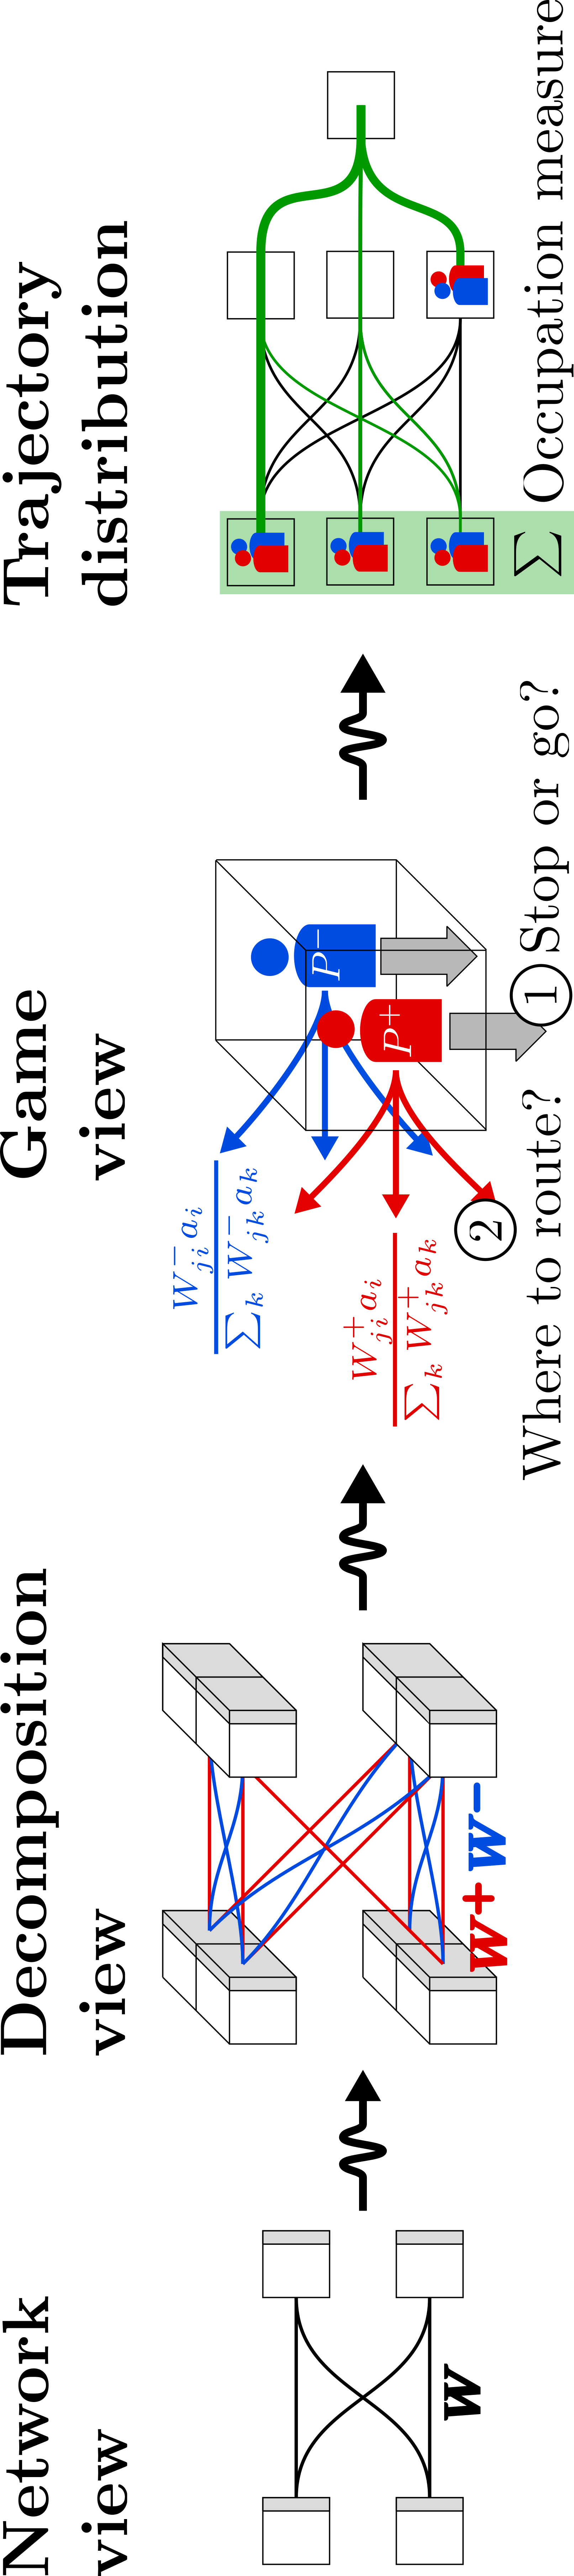
\includegraphics[angle=270,width=0.86\textwidth]{figures/ptnb_v2/main_figure.png}
\caption[The backward pass as a two-player game]{The backward pass as a two-player game. The Stopping Decomposition splits every weight by
sign, $W = W^+ - W^-$; at each state of the extended graph the players decide (1) stop or continue
and (2) where to route. Their equilibrium policies induce a distribution over backward
trajectories, and its signed discounted occupation measures at the input states recover the
attribution map.}
\label{fig:game_trajectory_overview}
\end{figure}

Oversight depends on the reliability of the evidence it uses. Parameter insensitivity, input dependence, perturbation fragility, and misleading modified-gradient structure~\parencite{Adebayo2018sanity,Kindermans2018PatternAttribution,Ghorbani2019fragile,Nie2018guided} can give false assurance about a model's visual dependencies. The two papers address complementary parts of this problem: the split representation exposes internal contributions and their derivative identities, while the game representation makes routing choices and distributions over calculations explicit. Numerical stabilization enables the former at depth; policy regularization, risk aversion, and extended action sets provide design choices for the latter. Hellinger diagnostics compare the resulting trajectory laws, complementing comparisons of their projected attribution maps. The experiments assess properties of these attribution methods; whether their use improves oversight or supports safer deployment remains a further empirical question.

Three research questions organize this combined account. \emph{What structure can be exposed without changing the network's function?} The decomposition framework connects monotone convex streams, sign-separated paths, and the polyhedral geometry of attainable gradients. \emph{What does a backward attribution actually calculate?} Derivative identities and game occupation measures relate local propagation rules to explicit global objects. \emph{How can these calculations support reliable inspection of vision models?} Stable implementations, controlled modifications of backward rules, and complementary evaluation criteria provide a basis for assessing what an attribution reveals and where its limitations lie.

\paragraph{Publication basis.}
This thesis brings together and extends two research works on which the thesis author is first author:
\begin{itemize}
    \item \emph{Hidden Monotonicity: Explaining Deep Neural Networks via their DC Decomposition}, coauthored with Georg Loho, was published at \textbf{CVPR 2026 and selected as a Highlight}~\parencite{hiddenMono}.\footnote{Official CVPR listing: \url{https://cvpr.thecvf.com/virtual/2026/poster/36564}.}
    \item \emph{Playing the Network Backward: A Game-Theoretic Attribution Framework}, coauthored with Jim Berend, Georg Loho, Sebastian Lapuschkin, and Wojciech Samek, is a \textbf{preprint}; this thesis uses arXiv:2605.06212v2, revised for AISTATS~\parencite{playingBackward2026}.
\end{itemize}
Their results are organized by the shared chain of questions: representation, backward semantics, method design, and evaluation. The experiments from each work remain separately identifiable. The thesis reuses their model-evaluation outputs, describes the implemented protocols, and recomputes the VOC uncertainty estimates with images as the resampling unit. It adds a common exposition of the decompositions, further mathematical connections, and a partial Lean formalization; Appendix~\ref{app:publication_provenance} records publication provenance and tool use.


\paragraph{Author's contribution.}
My principal contributions to the two underlying papers were developing the
theory, developing and conducting the experiments, and writing all appendices
and most of the paper text outside the introductions. These contributions were developed in
collaboration with the coauthors listed above. Appendix~\ref{app:author_contribution}
distinguishes this work from the subsequent integration and formalization in
the thesis.

\section{Contributions of This Thesis}\label{sec:contributions}

The contributions of this thesis are the following.

\begin{enumerate}
    \item \textbf{A general framework of network decompositions.}
    Chapter~\ref{ch:decompositions} introduces a \emph{network decomposition} and its \emph{validity}: a lift of a network into a pair of non-negative streams, propagated by non-negative maps $\Wsig{l}{+}, \Wsig{l}{-}$ and pairwise activations, whose difference recovers the original computation at every layer. Within it the thesis constructs a whole family --- the mixing family $\fmix$ interpolating between maximum- and minimum-based pair activations, the stopping decomposition $\fstop$, and regularized decompositions $\freg$ whose entropy-regularized member $\fsoft$ yields sigmoid-gated soft splits. The classical \ac{dc} split $f = g - h$ is the $\eta = 1$ endpoint of the mixing family rather than an isolated trick, and a splitting theorem for activations with integrable curvature extends the construction beyond \ac{relu} to GELU, Swish, tanh, sigmoid, and softplus networks.

    \item \textbf{A numerically stable \ac{dc} decomposition of \ac{relu} networks and \acp{cnn}.}
    A naive split can grow rapidly with depth while its difference stays bounded, so floating-point cancellation destroys the signal. Chapter~\ref{ch:decompositions} develops stabilization through transformations of the split activations and propagated signals. The exact convex representation extends to convolutions, convexity-preserving max-pooling, average pooling, fixed-statistic batch normalization, residual connections, and fixed dropout masks. The evaluated implementation additionally uses input-dependent recentering, cache correction, and optional winner-takes-it-all pooling. These procedures target forward reconstruction and usable backward signals; the individual stabilized streams do not inherit all convexity and monotonicity guarantees of the original representation.

    \item \textbf{A game-theoretic reformulation of the backward pass.}
    Chapter~\ref{ch:game_theory} reinterprets the stopping decomposition as a two-player zero-sum stopping game on an extended network graph, adapting the ReLU Net Game of \textcite{Gaubert2025}: layers are rounds, neurons states, sign switches hand the turn to the opponent, and the network output is the game value. Backward attribution is represented by \emph{signed discounted occupation measures over game trajectories}: propagation rules are equilibrium policies of the players $P^+$ and $P^-$, and attribution maps discounted occupation measures of that distribution. Two games anchor the theory --- the \ac{sg}, whose occupation measures recover the Jacobian, and the entropy-regularized \ac{rg}, recovering the full $\alpha\beta$-\ac{lrp} family --- giving the two methods a shared trajectory-space representation. These are representation theorems: the architecture alone does not determine a unique game or discount. The trajectory-space view of Chapter~\ref{ch:trajectory} further yields a Hellinger distance between normalized backward \emph{routing laws}, detecting routing changes that pixel-space sanity checks \parencite{Adebayo2018sanity} may obscure, and analytical \emph{modes} --- risk aversion, action-space augmentation, policy regularization --- mapping back to principled backpropagation rules.

    \item \textbf{New attribution methods and benchmark evaluations.}
    Chapter~\ref{ch:saliency} builds three attribution methods on the split representation: SplitCAM, a LayerCAM-inspired \parencite{Jiang2021LayerCAM} \ac{cam} method on the split-streams; SplitLRP, an adaptation of \ac{lrp} \parencite{Bach2015} to the split-pair; and SplitGrad, a gradient method exploiting the improved signal flow. Evaluated with the Quantus suite \parencite{Hedstrom2023} on VGG-16 \parencite{Simonyan2015} and ResNet-18 \parencite{He2016resnet} over ImageNet-S \parencite{Gao2022imagenets}, they show configuration-dependent gains in localization and Selectivity, with trade-offs in Pixel Flipping and robustness (Chapter~\ref{ch:experiments}). On ResNet-18, Guided Grad-CAM retains the highest reported Attribution Localization, and SplitCAM's Selectivity advantage over Guided Backprop is $0.014$. The chapter also develops directly trained difference-of-convex input neural networks and evaluates their stream sensitivities on MNIST (Section~\ref{sec:dcinns}).


    \item \textbf{A tropical-geometric interpretation and Imaginative Polytopes.}
    The tropical foundations (Section~\ref{sec:tropical_polyhedra_foundations}) place the decomposition in the polyhedral-geometry view of \ac{relu} networks \parencite{Zhang2018,Misiakos2022}: the split-streams $g$ and $h$ are the two tropical polynomials whose difference the network computes, their Newton polytopes evolving across layers by Minkowski sums and convex hulls. The thesis introduces \emph{Imaginative Polytopes} and proves that their vertices encode the attainable gradients of the split-streams, giving them an interpretation as learned visual prototypes and counterfactual feature profiles.

    \item \textbf{Extension to attention mechanisms and Transformers.}
    Chapter~\ref{ch:transformers} gives a recursive DC construction for deterministic Transformers of arbitrary finite depth, including signed attention projections, exact softmax, and LayerNorm with positive epsilon. Its streams are convex and monotone on non-negative doubled inputs and recover the full forward map exactly; numerical stability remains a separate issue. A distinct oracle-player construction treats the realized QK-softmax as a reference policy for conditioned Value routing. On ViT-B/16 \parencite{Dosovitskiy2021vit}, a selected game-derived attribution mode improves localization, with the selected configuration also evaluated on Pascal VOC without re-tuning. Pointing Game, Top-$k$ overlap, faithfulness, and robustness reveal distinct trade-offs; the revised evaluation reports independently validation-selected localization and faithfulness configurations, confidence intervals, and paired tests. These empirical results concern conditioned attribution, not the new full Transformer DC algorithm.
\end{enumerate}

\section{Positioning within the Literature}\label{sec:related_work}

This section positions the thesis along its three research questions; it is brief, since dedicated related-work discussions open the chapters where the material is developed --- games and propagation rules in Section~\ref{sec:related_work_games} and transformer interpretability in Section~\ref{sec:related_work_transformers}.

\paragraph{What structure is hidden inside a trained network?}
The idea that sign-constrained networks are the interpretable core of deep learning runs from monotonic networks \parencite{Sill1997_MonotonicNetworks,Daniels2010_MonotoneNN} through certified and lattice-based monotone models \parencite{Liu2020CertifiedMonotone,Gupta2016MonotoneLattice,Sivaraman2020_COMET,Nguyen2023_MonoNet,Runje_2023} to \acp{icnn} \parencite{Amos2017} and convex network calculus \parencite{Bach2017ConvexNN,Calafiore2019DLSE,sivaprasad2021curious}. \ac{dc} decompositions bridge this to unconstrained networks: classical \ac{dc} programming \parencite{Tao1997_DCProgramming,LeThi2018DCA,Sriperumbudur2009CCCP} and the representation theory of piecewise-linear functions as differences of convex ones \parencite{Melzer1986_PLasDC,Kripfganz1987_PWAasDC,Zalgaller2000_DCRepresentation,Griewank2020_PolyhedralDCDecomposition,Schlueter2021_ConvexDecompPAF,Koutschan2024_MinimalArity,Kazda2024_LP_DCPLA,Brandenburg2025_DecompositionPolyhedra} guarantee the split exists; \textcite{Awasthi2023DCNN} and \textcite{Siahkamari2020_DCRegression} construct essentially the split used here, for training and regression, and CDiNN-type architectures make the difference structure trainable \parencite{Sankaranarayanan2021CDINN,Chen2025_RCDiNN}. None confronts the numerical instability of the split or applies it to explanation, where this thesis departs. The geometric reading rests on the identification of \ac{relu} networks with \ac{cpwl} maps and tropical rational functions \parencite{Arora2018,Zhang2018,BalestrieroBaraniuk2018MadMax,Montufar2022,Misiakos2022,phuong2020functional,Hertrich2023,huchette2025deeplearningmeetspolyhedral}; the Newton-polytope perspective is developed in Section~\ref{sec:tropical_polyhedra_foundations}.

\paragraph{When can explanations be trusted?}
The attribution toolbox spans gradient saliency \parencite{Simonyan2014}, deconvolution and guided backpropagation \parencite{ZeilerFergus2014,Springenberg2015}, \ac{lrp} and Deep Taylor decomposition \parencite{Bach2015,Montavon2017DeepTaylor,Montavon2018}, \ac{cam} variants \parencite{Selvaraju2017,Chattopadhay2018,Jiang2021LayerCAM}, axiomatic methods \parencite{Sundararajan2017,Shrikumar2017}, noise averaging \parencite{Smilkov2017}, and perturbation- or surrogate-based explanations \parencite{Ribeiro2016,FongVedaldi2017,LundbergLee2017,Kolek2023_ShearletX,Fel2023_EVA}. A wave of critiques sharpened the trust question: sanity checks reveal parameter insensitivity \parencite{Adebayo2018sanity}, explanations can be fragile or manipulable \parencite{Ghorbani2019fragile,Dombrowski2019ManipulatedExplanations,AlvarezMelis2018robustness}, modified backward rules can produce structure unrelated to the model \parencite{Nie2018guided,sixt2020whenexplanationslie}, and input dependence confounds attribution \parencite{Kindermans2018PatternAttribution}. In response, evaluation frameworks such as Quantus \parencite{Hedstrom2023} operationalize faithfulness, localization \parencite{Zhang2018pointinggame}, robustness, and complexity \parencite{Bhatt2020complexity,Yeh2019} as measurable desiderata --- the standard this thesis holds its methods to in Chapter~\ref{ch:experiments}. The thesis' answer is structural rather than post hoc: attribution is computed on a representation (the split-pair) in which evidence cannot cancel invisibly, or derived from a game whose trajectory distribution records normalized backward routing and whose signed discounted occupation measures recover attribution, so sanity-check failures can be studied at both the trajectory and pixel levels (Chapter~\ref{ch:trajectory}); their different responses to randomization do not by themselves establish explanation faithfulness.

\paragraph{How can attribution be made stable?}
The closest precursor to the game framework is the ReLU Net Game of \textcite{Gaubert2025}, which identifies forward evaluation with the value of a zero-sum stopping game but connects it neither to the backward pass nor to attribution. Related stochastic views of relevance flow include Excitation Backprop's absorbing Markov chain \parencite{Zhang2018pointinggame}, which the \ac{sg} generalizes by adding an opponent, and the \ac{nrm} framework \parencite{Xiong2026nrm}, a signed-measure calculus over walks compared with our trajectory distributions in Section~\ref{sec:nrm_comparison}. Shapley-value methods \parencite{LundbergLee2017} play a \emph{different}, cooperative game over input coalitions in a black-box setting, complementary to the white-box backward game here. Stability itself has been approached via curvature reduction with softplus activations \parencite{Dombrowski2020} --- recovered here as entropy regularization of the stop decision --- and via risk-sensitive control \parencite{zhang2021risk} motivating the risk-averse game modes. On transformers, attention rollout and flow \parencite{Abnar2020attention}, transformer-\ac{lrp} \parencite{Chefer2021ICCV,Chefer2021GenericAttention,Ali2022AttnLRP,Achtibat2024AttnLRP}, and artifact-aware constructions \parencite{Wrobel2024,darcet2024vision} define the state of the art Chapter~\ref{ch:transformers} engages with; Section~\ref{sec:related_work_games} and Section~\ref{sec:related_work_transformers} give the full accounts. For visual inspection and attribution-guided correction~\parencite{Pahde2023R2R}, instability can obscure unwanted dependencies and misdirect subsequent interventions.

\paragraph{Outline.}
Chapter~\ref{ch:foundations} assembles the foundations: network notation, \ac{cpwl} mappings, convexity and monotonicity, \acp{mdp} and zero-sum games --- including the ReLU Net Game of Gaubert and Vlassopoulos --- and the tropical geometry of the split with the Imaginative-Polytope picture. Chapter~\ref{ch:decompositions} develops the decomposition framework, the smooth-activation splitting theorem, numerical stabilization, and the \ac{cnn} extension; Chapter~\ref{ch:game_theory} the two-player stopping and routing games, with gradients and $\alpha\beta$-\ac{lrp} recovered as equilibrium occupation measures; Chapter~\ref{ch:transformers} the extension and implementation on multiplicative operations and \acp{vit}; and Chapter~\ref{ch:saliency} the split methods SplitCAM, SplitLRP, and SplitGrad, inherently interpretable difference-of-convex architectures, and the attribution modes. Chapter~\ref{ch:experiments} reports the evaluation on ImageNet-S and Pascal VOC across VGG-16, ResNet, and ViT-B/16; Chapter~\ref{ch:trajectory} develops the trajectory-distribution view and its Hellinger diagnostics; and Chapter~\ref{ch:conclusion} concludes with future directions from \acp{llm} to hardware-level acceleration.
